\chapter{Realisierung}
% Dies ist das Hauptkapitel Ihrer Arbeit! Hier wird die Umsetzung der eigenen Ideen und Konzepte
% (Kapitel 3) anhand der gewählten Methoden (Kapitel 4) beschrieben, inkl. der dabei aufgetretenen
% Schwierigkeiten und Einschränkungen.
Die Realisierung lässt sich in drei Phasen unterteilen.

In der ersten Phase werden grundlegende Entscheidungen getroffen und die Basis der Arbeit implementiert.
Am Ende der ersten Phase existiert ein Prototyp,
welcher bei allen Komponenten des System über die minimalen Funktionen verfügt. (TODO verweis )

Wie im Kapitel Vorgehen beschrieben (TODO), folgen darauf zwei weitere Phasen,
in welche neue Anforderungen des Auftraggebers umgesetzt werden.

\section{Phase 1: Grundlegende Designentscheidungen}
In der ersten Phase wurden die Grundlagen des Systems entwickelt.
Technologien wurden evaluiert, ein Datenbankschema erstellt und eine geeignete Systemarchitektur entwickelt.
Auch die \ac{CI/CD} Infrastruktur wurde direkt zu Beginn aufgesetzt.

TODO: Idee: Architektur und so, also alles was grundlich erklärt wird, nicht bei Phase 1 sonder zuvor erklären.
Damit Phase 1 nicht viel grösser als die anderen ist. In Einleitung entsprechend darauf hinweisen.

\subsection{Evaluation der Technologien}
\label{p1:evaluation_tech}
Die Evaluation der Technologien lässt sich grundsätzlich in Frontend und Backend unterteilen.
Für das Projektteam war es wichtig, dass diese beiden Teile unabhängig von einander evaluiert und entwickelt werden können.
Die Kommunikation zwischen beiden wird mit einer \ac{REST} \ac{API} realisiert, da dies in der Aufgabenstellung verlangt wird. TODO Verweis

\subsubsection{Frontend}
Vorgabe für das Frontend war zu Beginn des Projektes lediglich,
dass sie von mobilen Endgeräte, also Smartphones, abrufbar sein sollte.
Dies lässt sich auf zwei Arten umsetzt:
\begin{itemize}
    \item Eine App entwickeln, welche auf dem Gerät installiert werden kann.
    \item Eine Webseite entwickeln, welche vom Gerät aufgerufen werden kann.
\end{itemize}
Die Entscheidung fiel auf letztere Art, also eine Webseite.
Die Gründe dazu sind:
\begin{itemize}
    \item Das Projektteam hat in der Vergangenheit bereits Webseiten entwickelt.
          Diese Erfahrungen warne positiv und zeigten, dass so in geringer Zeit gute Resultate erreicht werden können.
    \item Eine Webseite schränkt die Zielplattform weniger ein als eine App.
          Bei einer App müsste bereits zu beginn eine einzelne Platform, wie bspw. Android oder iOS ausgewählt werden.
          Webseiten können auf diversen Plattformen dargestellt werden.
    \item Eine Person des Projektteams besuchte parallel zu diesem Projekt das Modul ``Datenvisualisierung``  an der Hochschule Luzern.
          Nebst den Grundlagen zu Datenvisualisierung wurde in diesem Modul auch die Anwendung des Visualisierungs-Frameworks D3.js \footnote{https://d3js.org/} vertieft.
          Da mit D3.js Grafiken für Webseiten erstellt werden können, lag es auf der Hand, das bereits gelernte auch in dieser Arbeit umzusetzen.
\end{itemize}

Um von den in \ref{state:frontend} erwähnten Vorteile eines Frontend Framework zu profitieren,
wurde ein passendes evaluiert.

Das Projekt Team hatte in der Vergangenheit bereits mit den Frameworks Angular \footnote{https://angular.io/}, Vue.js \footnote{https://vuejs.org/} und React.js \footnote{https://reactjs.org/} gearbeitet
und unterschiedliche Erfahrungen gesammelt, sieht sich jedoch als Anfänger im Bezug auf Webentwicklung.
Die Entscheidung fiel auf React.js, da dies sich für Anfänger eignet und im Zusammenspiel mit weiteren Frameworks eingesetzt werden kann \parencite{react_angular_vue}.
Letzteres ist wichtig, da das zuvor erwähnte D3.js Framework für die Visualisierungen verwendet werden soll.

TODO evaluation MUI


\subsection{Backend}
Bei er Auswahl des Technologiestacks wurde auf verschiedene Aspekte geachtet.
Zum einen sollte das Frontend unabhängig vom Backend entwickelt werden können.
Aus diesem Grund wurde für die Kommunikation, wie in Kapitel \ref{konzepte:api-kommunikation}
bereits beschrieben, eine \ac{REST} \ac{API} verwendet.
Auf die genaue Definition der \ac{API} wird in den nächsten Abschnitten noch genauer eingegangen.

Für die Implementation des Backends gibt es unzählige Technologien die man für eine \ac{CRUD}
Applikation verwenden kann (Siehe Kapitel \ref{state:backend}). Für dieses Projekt sollte
eine \ac{REST} \ac{API} implementiert werden können. Und die Datenbank soll über ein \ac{ORM}
abstrahiert werden können. Dies hat den Vorteil, dass die eigentliche Datenbanktechnologie
keine grosse Rolle spielt. Das \ac{ORM} abstrahiert die Tabellenstruktur mittels
Objekten im Sourcecode. Als Backend kann beispielsweise zum Testen und Entwickeln
eine Sqlite\footnote{https://www.sqlite.org/index.html} Datenbank verwendet werden.
Der gleiche Sourcecode kann danach in der Produktion auf eine PostgreSQL\footnote{https://www.postgresql.org/}
Datenbank zugreifen um besser zu skallieren.
Natürlich soll auch ein \ac{MQTT} Framework in der gewählten Technologie zur verfügung stehen
damit die Messdaten der Stromzähler empfangen und in die Datenbank abgespeichert werden können.

Python bietet für jedes dieser Anforderungen gleich mehrere Frameworks an. Mit Python können sehr
schnell Prototypen erstellt werden. Es eignet sich aber auch für grosse Produktivsoftware.
Einige der wohl Bekanntesten Programme wie YouTube, Instagram, Spotify oder Reddit sind
in Python geschrieben. \cite{popular_python_sw}

Bei der Implementation des Frontends wurde wie in Kapitel \ref{state:frontend} beschrieben
anhand der State of Js Umfragen React\footnote{https://reactjs.org/} verwendet.
Um nicht das ganze Benutzerinterface selber gestalten zu müssen, wurde eine Material Design\footnote{https://material.io/design}
Library verwendet.

Um die Applikation für die Entwicklung lokal aufzusetzen, zu testen oder zu Deployen wurde dazu
Podman verwendet (Siehe Kapitel \ref{state:deployment}).


\subsection{Systemarchitektur}
\label{architekturentscheidung}

In dieser Arbeit wird keine Microservice Architektur im klassischen Sinne verwendet. (Siehe Kapitel \ref{konzepte:microservices})
Die einzelnen Komponenten werden zwar in separaten Container deployt (Abbildung: \ref{fig:smic-arch})
besitzen jedoch keine eigene Datenbank.
Das hat den Vorteil, dass weniger Overhead implementiert werden muss (mittels Message Queue)
und das Datenbankschema kann zentral in der Datastore Library einmal definiert
und dann in den verschiedenen Komponenten wiederverwendet werden.


\begin{figure}[h]
    \centering
    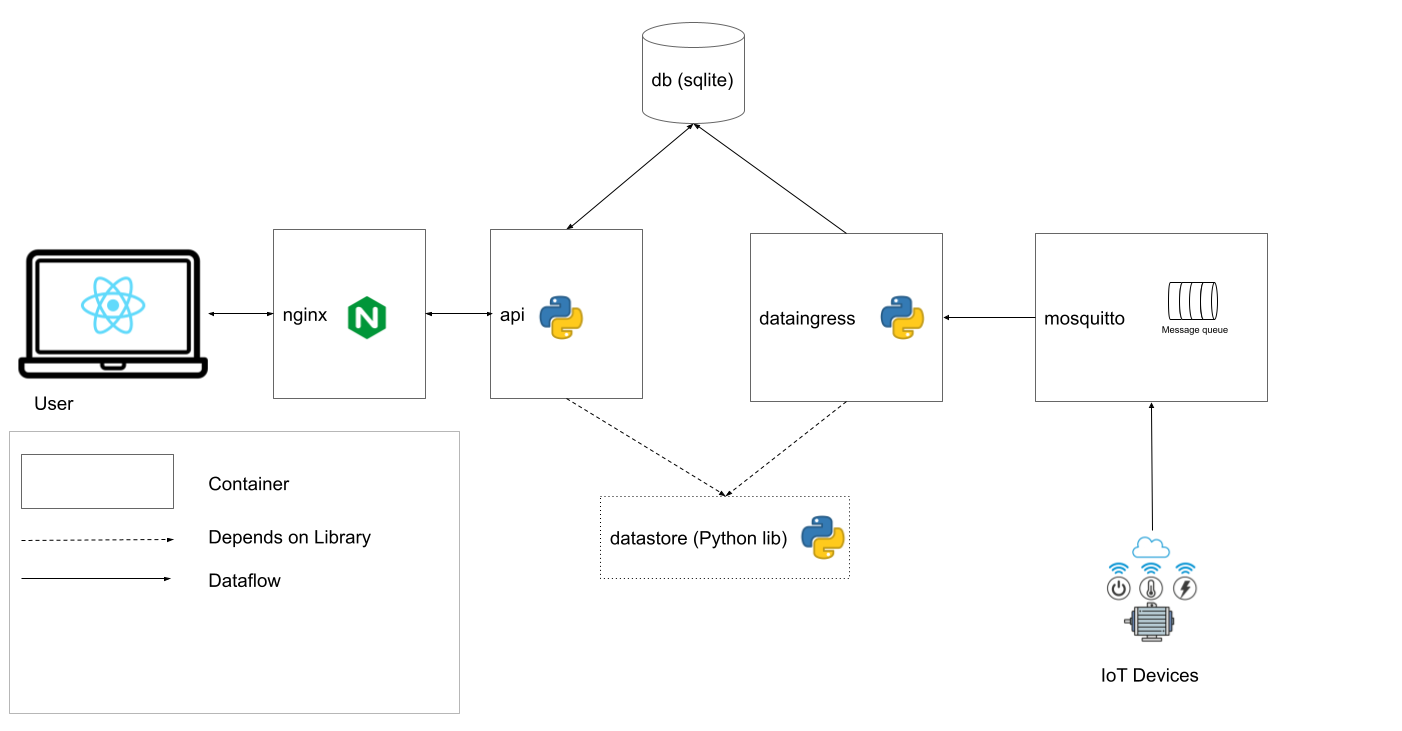
\includegraphics[width=1.0\textwidth]{gfx/smic-arch}
    \caption{
        Schematische Darstellung der in diesem Projekt verwendeten Architektur
    }
    \label{fig:smic-arch}
\end{figure}

Die Abbildung \ref{fig:smic-arch} zeigt die in diesem Projekt verwendete
Architektur auf. Hier noch einige Informationen zu den einzelnen Komponenten:


\begin{itemize}
    \item \texttt{nginx}:
          Alle Anfragen des Endbenutzers werden über einen Nginx Server
          entgegengenommen. Dieser liefert dann dem Benutzer die React WebApp
          oder leitet Anfragen an die \ac{API} weiter.

    \item \texttt{api}:
          Die \ac{API} verarbeitet Datenanfragen der React WebApp. Sie gibt
          beispielsweise die Stromzählerdaten eines Tages zurück.

    \item \texttt{datastore}:
          Der datastore ist eine Python library, die das Datenbankschema mittels \ac{ORM} festlegt.
          Sowohl die \ac{API} als auch der dataingress greifen auf die Datenbank zu
          und verwenden somit die datastore library.

    \item \texttt{dataingress}:
          Der dataingress arbeitet die von den \ac{IoT} Geräten gesendeten
          Stromzählerdaten ab und speichert diese in die Datenbank.

    \item \texttt{mosquitto}:
          Mosquitto ist der in dieser Arbeit verwendete \ac{MQTT} Broker.
\end{itemize}

Ein weiterer grund für die Entscheidung einer geteilten Datenbank ist,
dass der \texttt{dataingress} keine Daten liest, sondern diese nur von
der \ac{MQTT} Queue abarbeitet und in die Datenbank schreibt.

Auf die einzelnen Komponenten wird später in der Realisierungsphase noch genauer
eingegangen.

\subsection{\ac{CI/CD}}

% TODO: move to stand der technik

Um das Projekt automatisch Testen zu können und eine Reproduzierbare Umgebung zu bauen,
wurde bereits zu Beginn eine \ac{CI/CD} Pipeline mit GitHub Actions\footnote{https://github.com/features/actions}
aufgebaut.
Die Entwickler sollen sich nicht nur um die Entwicklung, sondern auch das automatische Bauen und Deployen der
Software kümmern. Dieser DevOps Gedanke hat den Vorteil, dass
theoretisch jedes kleine Feature und jeder Bugfix direkt automatisiert getestet
wird und danach (wenn die Tests erfolgreich waren) auf das Produktivsystem
Deployt werden kann. \cite{what_is_devops}
zudem ist für jeden Entwickler das Bauen und Ausführen des Projektes gleich und
reproduzierbar. Dies erspart das Suchen von unnötigen Fehlern die auf unterschiedlich
konfigurierten Entwicklungsmaschinen auftreten können.

\begin{figure}[h]
    \centering
    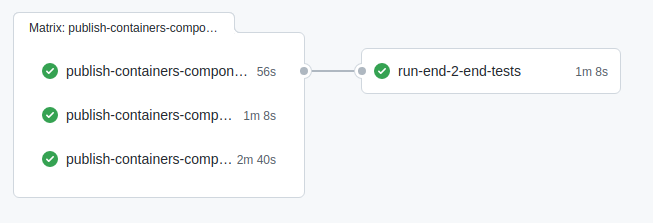
\includegraphics[width=1.0\textwidth]{gfx/ci-env}
    \caption{
        Visualisierung der GitHub Actions Pipeline mit zwei aufeinanderfolgenden Stages.
        Zuerst werden die einzelnen Komponenten (Siehe \ref{fig:smic-arch}) gebaut und
        anschliessend getestet.
    }
    \label{fig:ci-env}
\end{figure}

Dank dieser \ac{CI/CD} Umgebung und der Verwendung von Podman, kann die gesamte Applikation
(Wie im Kapitel \ref{architekturentscheidung} beschrieben) mit einem
Befehl gebaut und gestartet werden.

\subsection{Verarbeitung und Visualisierung von Stromzählerdaten}
TODO Kapitel Aufteilung überdenken...
In einer ersten Phase werden laut der Aufgabenstellung \ref{aufgabenstellung} Stromzähler
Messdaten per \ac{MQTT} empfangen und in eine Datenbank gespeichert.
Diese gespeicherten Daten werden dann in einer WebApp visualisiert und dem Benutzer
angezeigt.

\begin{figure}[h]
    \centering
    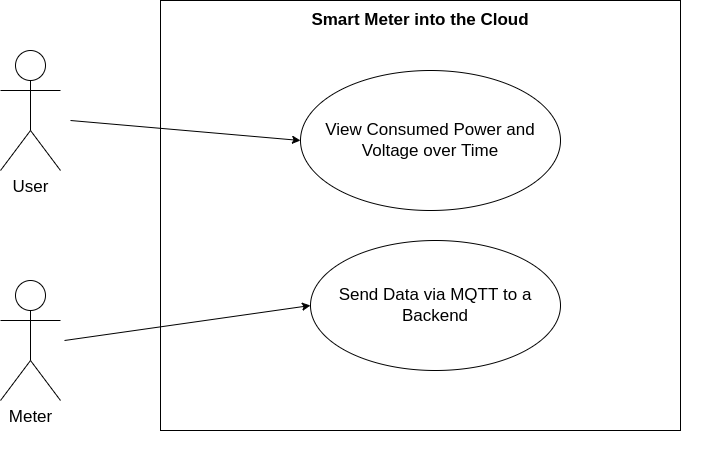
\includegraphics[width=1.0\textwidth]{gfx/usecase1}
    \caption{
        UseCase Diagramm der Verarbeitung und Visualisierung von Stromzählerdaten.
    }
    \label{fig:usecase1}
\end{figure}

\subsection{Frontend und Backend Abstraktion}

Damit die Arbeit von Frontend und Backend aufgeteilt werden kann, wurde zuerst
die \ac{API} Schnittstelle definiert. Für die Implementierung im Backend
stand die Entscheidung zwischen Flask\footnote{https://flask.palletsprojects.com/en/2.0.x/}
und FastAPI\footnote{https://fastapi.tiangolo.com/}.
Flask ist ein simples Web Framework mit dem \ac{API}s aber auch Server Side Rendering \cite{flask_server_side}
gemacht werden kann. FastAPI ist ein typisiertes Framework das darauf spezialisiert ist
\ac{REST} \ac{API}s zu implementieren. FastAPI ist ähnlich aufgebaut wie Flask aber auf den
\ac{API} Bereich spezialisiert. Die Dokumentation wird auch automatisch generiert.
FastAPI eignet sich perfekt um die \ac{API} zwischen Frontend und Backend zu implementieren.

\begin{figure}[h]
    \centering
    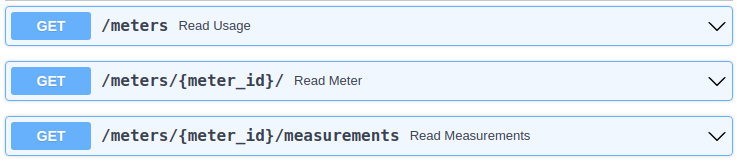
\includegraphics[width=1.0\textwidth]{gfx/api-visualization}
    \caption{
        \ac{API} Definition für die Visualisierung von Stromzählerdaten
    }
    \label{fig:api-visualization}
\end{figure}

Wie in Abbildung \ref{fig:api-visualization} dargestellt, besteht die \ac{API} der Stromzähler
und Messdaten ausschliesslich aus Abfragen. Die zu speichernden Daten kommen dann (wie im nächsten
Abschnitt erklärt) aus den \ac{MQTT} Daten der Stromzähler selbst.

\begin{figure}[h]
    \centering
    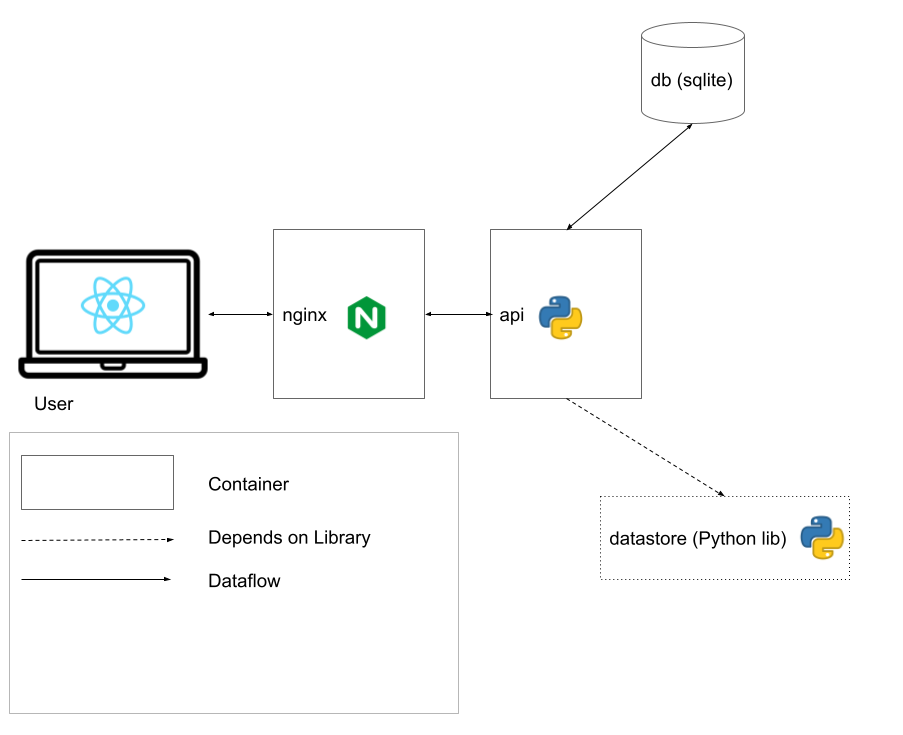
\includegraphics[width=0.8\textwidth]{gfx/sim-arch-api}
    \caption{
        Architektur der \ac{API} zwischen Frontend und Backend
    }
    \label{fig:arch-visualization-front-back}
\end{figure}

Sobald die WebApp von einem Benutzer aufgerufen wird, lifert der Nginx Server
die WebApp per \ac{HTTP} request aus. (Abbildung \ref{fig:arch-visualization-front-back})
Wenn der Benutzer (in diesem Fall über das React Web Frontend) danach die Messdaten seines
Stromzählers abfragen will, wird ebenfalls eine Asynchrone \ac{HTTP} Anfrage an die Backend \ac{API} gemacht.
Die Abfrage landet dann beim Nginx und wird an das Python FastAPI Backend weitergeleitet.
Dieses Python Backend führt danach eine SQL Abfrage via \ac{ORM} auf der Datenbank aus.
Um die Daten im Web Frontend anzeigen zu können, werden sie noch \ac{JSON} serialisiert
und zurück an die WebApp gesendet.

Die datastore Python Library stellt der \ac{API} das Datenbankschema zur Verfügung,
damit das \ac{ORM} die Abfragen an die Datenbank machen kann.
Als \ac{ORM} Framework wird sqlmodel\footnote{https://github.com/tiangolo/sqlmodel} verwendet.
Sqlmodel wird vom gleichen Entwickler wie FastAPI maintaint und bietet eine gute Integration.

Da nun das Datenmodell (in der datastore Library) und die \ac{API} definiert wurden,
kann das Web Frontend unabhängig vom Verarbeiten der \ac{MQTT} Daten gemacht werden.

\subsection{Implementation der Backend \ac{API}}

Wie alle Python Komponenten dieses Projektes wird auch das Backend \ac{API}
als Python Poetry\footnote{https://python-poetry.org/} Projekt implementiert.
Poetry verbessert das Paketmanagement von Python erheblich gegenüber Setuptools
und pip. \cite{python_poetry}
Dadurch ist es auch einfacher die Applikation als Container zu bauen und
damit einen reproduzierbaren Build zu garantieren.

Die Datenbankanbindung kann per Datenbank \ac{URI} dem sqlmodel Framework
mitgegeben um zu bestimmen auf welche Datenbank zugegriffen werden soll.



\subsection{\ac{MQTT} Datenverarbeitung}

Die Daten der Stromzähler werden per \ac{MQTT} an den Broker gesendet. \ref{state:mqtt}

\begin{figure}[h]
    \centering
    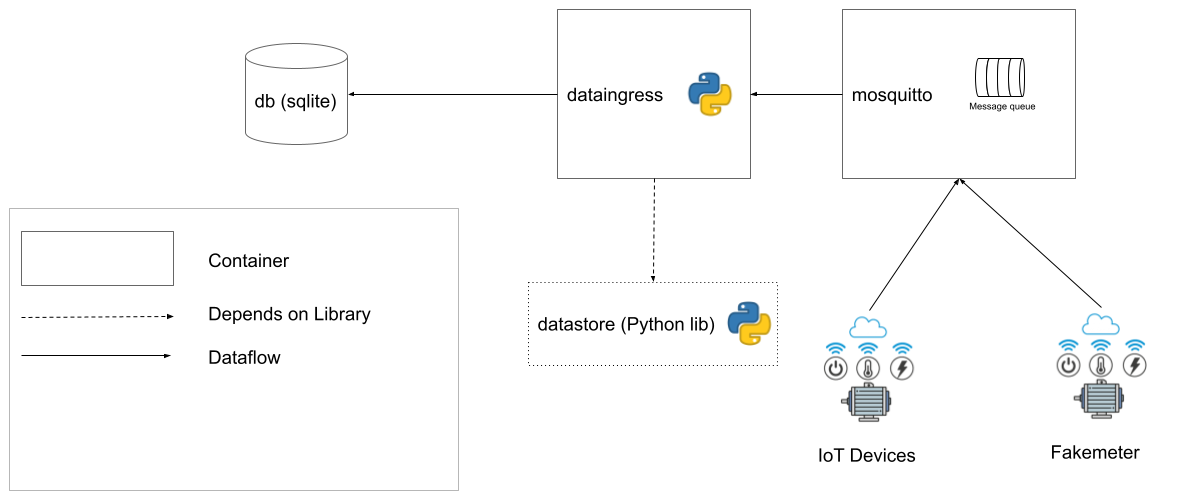
\includegraphics[width=1.0\textwidth]{gfx/smic-arch-mqtt}
    \caption{
        Architektur des \ac{MQTT} Messagebroker und des Dataingress welcher die
        empfangenen Nachrichten in die Datenbank persistiert.
    }
    \label{fig:arch-mqtt}
\end{figure}

Der Dataingress (ebenfalls ein Python Poetry projekt) registriert sich dann auf die von
den Stromzählern gesendeten Events und arbeitet diese ab. Das Empfangen und Abarbeiten, bzw.
in die Datenbank schreiben wird von unterschiedlichen internen Komponenten übernommen.
Beim Abarbeiten wird zudem, falls ein Datensatz nicht prozessiert werden kann dies noch
einmal versucht. Beispielsweise kann die Datenbank noch nicht bereit sein.\footnote{
    Das kann beispielsweise passieren, wenn die Datenbank neu gestartet wird nach einem update.
}
Dadurch soll möglichst verhindert werden, dass eingehende Messdaten verloren gehen.

Auch der Dataingress verwendet die Datastore Python Library. Dies stellt sicher,
dass die \ac{API} und er Dataingress das gleiche Datenbankformat verwenden da
die Datenbank ja zwischen den beiden Applikationen geshart ist.

\begin{figure}[h]
    \centering
    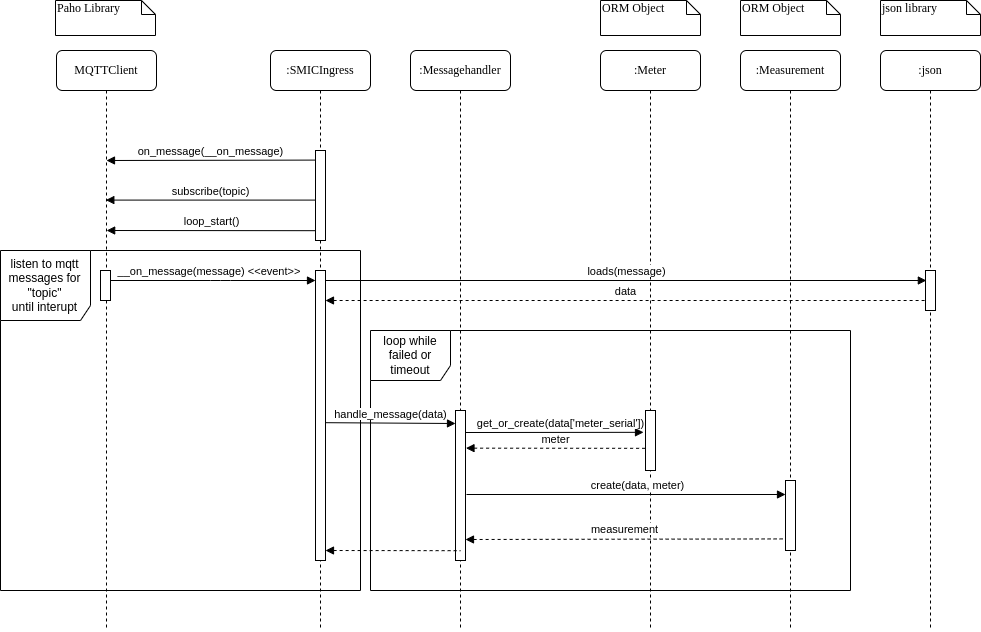
\includegraphics[width=1.0\textwidth]{gfx/dataingress-sequence}
    \caption{
        Das Sequenzdiagramm zeigt auf wie der Dataingress die \ac{MQTT} Messages
        von den Stromzählern abarbeitet und in die Datenbank persisitiert.
    }
    \label{fig:dataingress-sequence}
\end{figure}

Im Sequenzdiagramm des Dataingress (Abbildung \ref{fig:dataingress-sequence}) wird aufgezeigt
wie \ac{MQTT} Messages vom Dataingress abgearbeitet werden.
Die Messages müssen zuerst \ac{JSON} deserialisiert werden, um in Python
gebraucht zu werden. Danach werden die Messdaten und allenfalls der
Stromzähler mit Serialnummer in die Datenbank gespeichert.

\subsection{Automatisierte End to End Tests}

Wie bereits in der Teststrategie \ref{teststrategie} erwähnt werden für dieses Projekt
hauptsächlich automatisierte End to End Tests implementiert.

Damit die Tests automatisiert ausgeführt werden können, wurde ein Stromzähler Simulator entwickelt.
Zwar wäre es theoretisch möglich gewesen auch einen echten Stromzähler für Tests zu verwenden,
jedoch ist es immer schwierig Automatisierungen mit Hardware zu machen. Zudem können
Daten bei physikalischen Geräten nur in Echtzeit und nicht schneller übertragen werden.
Durch diesen "Fakemeter" konnten Daten mehrerer Tage innert weniger Sekunden oder Millisekunden
an das Backend (den Dataingres \ref{fig:dataingress-sequence}) gesendet werden.

Der Stromzählersimulatof verfügt sowohl über eine Python Schnittstelle als auch über
ein Command Line Interface. Dies ist besonders während der Entwicklung nützlich:

\begin{verbatim}
poetry run fakemeter --meter-serial METER_SERIAL \
  VOLT_1 VOLT_2 VOLT_3 POWER
\end{verbatim}


\subsection{Benutzerschnittelle}
Um den Anwendungsfall, ``Einsehen von Spannungswerten über Zeit`` (Abbildung \ref{fig:usecase1}) zu erfüllen,
wurde eine minimale Benutzerschnittstelle entwickelt, welches lediglich einen Graphen darstellt.
Dieser stellt den Verlauf der Spannungswerte über die Zeit dar.
Der Aufbau der Benutzerschnittstelle basiert auf der Skizze,
welche im Kapitel \ref{konzepte:entwurf-benutzerschnittstelle} vorgestellt wurde.
Auf die dort angedachten Filter-Komponenten wurde bewusst verzichtet, da diese für das erreichen des
minimalen Prototypen noch nicht benötigt werden.

Die gezeigten Daten werden über die \ac{REST} \ac{API} geladen und mit Hilfe von d3.js dargestellt.


\subsection{Schwierigkeiten}
Das gewählte Frontend Framework, React, war für das Projektteam grösstenteils neu.
Somit wurde in dieser ersten Phase viel Zeit in das Erlernen der Grundlagen von React investiert.
Kleine Programmierfehler führten aufgrund der fehlenden Erfahrung und Routine zu grösseren Schwierigkeiten.
Durch die Hilfe von Freunden, Mitstudienenden und Hilfsmittel im Internet liessen sich diese meistern
und die erste Phase im geplanten Zeitrahmen abschliessen.

\section{Phase 2: Erste Rückmeldungen des Auftraggebers}
Screenshot der ersten version
Rückmeldungen:
- grundsätzlich zufrieden
- Mobile nicht weiter zentral, Fokus auf Dashboard, Desktop

Neue Anforderungen:
Range/Zähler auswählen sowie typ der Daten
echte Daten automatisiert einspielen
THD und Power zusätzlich zu Spannung

\subsection{Änderungen der Anforderungen}
Aufzählen was geändert wurde
\subsection{Schwierigkeiten}
Schwierigkeiten während der zweiten Phase

\section{Phase 3}
TODO Einleitung
Dabei sind folgenden Rückmeldungen entstanden:
\begin{itemize}
    \item Die für Desktops optimiert Benutzerschnittelle entspricht den Vorstellungen und wirkt intuitiv.
    \item Da vom Auftraggeber keine echten \ac{THD} Werte zur Verfügung gestellt werden können,
    können diese weggelassen werden.
    \item Die Applikation soll unm die in der Aufgabenstellung (Anhang \ref{anhang:aufgabenstellung}) beschrieben Anforderung:
    ``Eine benutzerdefinierte Zeitspanne der Messwerte mittels vorgegebener 
    Labels beschriften. Bsp.: («Backofen war von 09:31 – 10:15 aktiv»)`` soll implementiert werden.
    \item Die Übertragung der Messdaten mittels \ac{MQTT} soll,
     wie bereits in der Aufgabenstellung (Anhang \ref{anhang:aufgabenstellung}) verlangt, mit \ac{TLS} verschlüsselt werden.
\end{itemize}

\subsection{TLS Verschlüsselung}

\subsection{Benutzerschnittstelle}
% \subsection{Labeling}
% - Labeling:
% Labels graphisch darstellen
% Labels mittels UI hinzufügen

\subsection{Schwierigkeiten}
TLS..


